\section{Theorie}
\label{sev:Theorie}

In dem folgenden Versuch geht es darum, einerseits die Funktionsweise und Inbetriebnahme
eines Helium-Neon-Lasers experimentell nachzuvollziehen. Anschließend werden durch
weitere Messungen mehrere Eigenschaften des Lasers untersucht. Dazu gehören die
Stabilitätsbedingungen, die Polarisation, die Wellenlänge sowie eine Untersuchung
der TEM-Moden.

Laser (Light Amplification by Stimulated Emission of Radiation)
sind unter anderem aufgrund ihrer hohen Intensität sowie der langen
Köhärenzlänge (ca. 11 km) interessant für verschiedene Bereiche der Medizin sowie
allgemein als Grundlage verschiedener Messmethoden.

Ein Laser besteht allgemein aus 3 grundlegenden Komponente. Dem aktiven Lasermedium,
dem Resonator sowie einer Pumpquelle, da zur Erzeugung das Prinzip des Optischen
Pumpens verwendet wird. Das Lasermedium wird dabei mithilfe der Resonatoren sowie
des optischen Pumpens so manipuliert, dass es zu einer Verstärkung des einfallenden
Lichtes kommt. Dieses Prinzip wird auch als selbsterregenden Oszillator bezeichnet.

\subsection{Grundprinzip des Laserns}
\label{sub:GrundLaser}

Ein Ergebniss der Quantenmechanischen Betrachtung ist, dass jedes Atom diskrete
Energieniveaus besitzt. Die Besetzungzahlen zweier verschiedener Niveaus $n\ua{1}$
und $n\ua{2}$ mit den Energien $W\ua{1}$ < $W\ua{2}$ sind
dabei gemäß der Maxwell-Boltzmann-Verteilung miteinander verknüpft:

\begin{equation}
  \frac{N\ua{2}}{N\ua{1}} = \frac{g\ua{2}}{g\ua{1}} \frac{\exp{(-W\ua{2}/k\ua{B}T)}}{\exp{(-W\ua{1}/k\ua{B}T)}}.
  \label{eqn:NRelation}
\end{equation}

$k\ua{B}$ ist dabei die Boltzmann-Konstante, $T$ die Temperatur und $g\ua{i}$
sind die zugehörigen statistischen Gewichte. Trifft nun ein Photon mit der Energie
des entsprechenden Überganges auf das Atom, so kann es absorbiert werde. Dabei
geht das Atom in einen höheren Zustand über, zum Beispiel vom Grundzustand in den
ersten angeregten Zustand. Geht es anschließend wieder in den Grundzustand über,
wird ein Photon emittiert, welches genau die Differenz beider Niveaus als Energie
besitzt:

\begin{equation}
  \hbar \omega = E\ua{2} - E\ua{1}.
\end{equation}

Passiert dies spontan, wird dies als spontanen Emission bezeichnet. Die Emission
kann allerdings auch durch Einstrahlen eines Photons erzeugt werden, so dass man
am Ende zwei Photonen mit der selben Energie, Phase und Ausbreitungsrichtung erhählt.
Bei diesem Vorgang handelt
es sich um die induzierte Emission. Die Vorgänge sind in Abbildung \ref{fig:Emission}
noch einmal grafisch dargestellt.

\begin{figure}
  \centering
  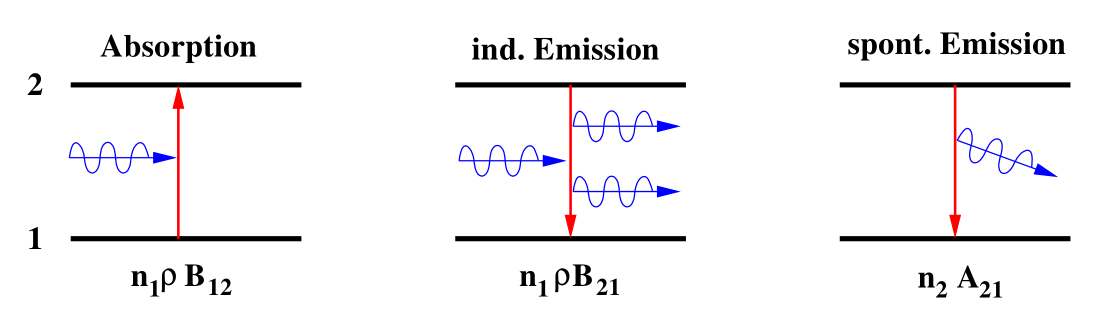
\includegraphics[width = \textwidth]{Pics/EmAb.png}
  \caption{Emission und Absorption. \cite{anleitung}}
  \label{fig:Emission}
\end{figure}

Die Wahrscheinlichkeit, mit der die verschiedenen Vorgänge zwischen zwei Niveaus
auftreten wird über die Einstein-Koeffizienten $B$ und $A$ bestimmt. Die Anzahl der
spontanen Emissionen pro Zeiteinheit lässt sich dann wie folgt berechnen, wobei
$A\ua{21}$ die Übergangswahrscheinlichkeit von Niveau $W\ua{2}$ in $W\ua{1}$ darstellt:

\begin{equation}
  n\ua{spon} = N\ua{2}A\ua{21}.
  \label{eqn:Nspon}
\end{equation}

Die Anzahl induzierter Emissionen pro Zeiteinheit ist mit $N\ua{2}$ über den
Einstein-Koeffizienten $B\ua{21}$ sowie dem Strahlungsfeld $ro$ verbunden:

\begin{equation}
  n\ua{ind} = N\ua{2}B\ua{21}\rho.
  \label{eqn:Nind}
\end{equation}

Durch eine ähnliche Relation lässt sich auch die Anzahl absorbierter Quanten pro
Zeiteinheit bestimmen:

\begin{equation}
  n\ua{abs} = N\ua{1}B\ua{12}\rho.
  \label{eqn:Nabs}
\end{equation}

Unter der Annahme, dass beide Niveaus nicht entartet
sind ($g\ua{1}=g\ua{2}$), gilt $B\ua{12} = B\ua{21}$. Somit lässt sich nun
$A\ua{21}$ bestimmen, so dass sich folgende Abhängigkeit ergibt:

\begin{equation}
  A\ua{21} = \frac{8\pi h}{c^3}B\ua{12}\nu^3.
  \label{eqn:A21}
\end{equation}

Im thermischen Gleichgewicht überwiegt dabei gemäß der Maxwell-Boltzmann-Verteilung
die Besetzung des Grundzustandes. Für die zum Lasern benötigte dauerhafte Verstärkung
des Strahlungsfeldes muss die induzierte Emission deutlich häufiger auftreten als
die spontane Emission. Dafür ist eine höhere Besetzung des angeregten Zustandes
nötig, welche auch als Besetzungsinversion bezeichnet wird. Diese wird durch das
optisches Pumpen realisiert.

Die Besetzungsinversion ist allerdings in einem reinen 2-Niveau-System wie es hier
verwendet wurde nicht realisierbar. Dies ergibt sich relativ schnell aus Gleichung
\eqref{eqn:NRelation}. Geht man von nicht entarteten Zuständen aus, kann lediglich
die Temperatur als Parameter beeinflusst werden. Selbst beim Limes T $\leftarrow$ $\infty$
kann lediglich ein Verhältniss von 50:50 erreicht werden. Zudem kann es auch damit
erklärt werden, dass bei einem Zwei-Nievau-System irgendwann die Wahrscheinlichkeit
für die induzierte Emission genauso hoch ist wie die für die Absorption, genau dann
wenn $n\ua{1}$ = $n\ua{2}$ gilt (siehe \eqref{eqn:Nind} und \eqref{eqn:Nabs}).


\subsection{Besetzungsinversion beim HeNe-Laser}

Beim HeNe-Laser wird die Besetzungsinversion des Lasermediums Neons nicht direkt erzeugt.
Stattdessen wird Helium vom Grundzustand in einen angeregten Zustand gehoben.
Da die Energiedifferenz zwischen den $2^1S\ua{0}$ und $2^3S\ua{1}$ Niveaus des Heliums
ungefähr der Differenz zwischen $3s$ und $2s$ Niveaus des Neons enstpricht, kann dieses
durch Stöße 2.Art in einen angeregten Zustand gehoben werde. Das Helium geht dabei
wieder in den Grundzustand über und kann anschließend erneut angeregt werden.
Somit kann eine Besetzungsinversion beim Neon erzeugt werden (siehe Abbildung \ref{fig:Inversion}).

\begin{figure}[h]
  \centering
  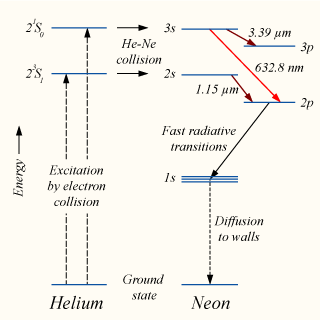
\includegraphics[width = 0.7\textwidth]{Pics/Niveaus.png}
  \caption{Besetzungsinversion beim HeNe-Laser. \cite{Inversion}}
  \label{fig:Inversion}
\end{figure}


\subsection{Resonatoraufbau und Stabilitätsbedingung}
\label{sub:ResStab}

Da die Verstärkung exponentiell mit der Länge des Lasermediums anwächst, wird bei
dem Laser ein Resonator verwendet. Dieser besteht im Grunde aus zwei Teilspiegeln,
wovon einer teilreflektierend und einer totalreflektierend ist, sowie dem Lasermedium
(siehe Abbildung \ref{fig:Resonator}). Durch die beiden Spiegel durchläuft der Strahl
mehrfach das Medium, wobei immer ein Teil an dem teildurchlässigem Spiegeln
ausgekoppelt wird. Für den Resonator können dabei verschiedene Spiegel benutzt werden.
Allerdings müssen für einen selbstanregenden Oszillator die Verluste möglichst gering
gehalten werden, was besonders durch konkave Spiegel optimal realisiert werden kann.
Ein Beispiel dafür ist der konfokale Resonator, bei dem die Spiegelbrennpunkte zusammenfallen.
Sind die enstehenden Verluste kleiner als die Verstärkung, so spricht man von einem
optisch stabilen selbsterregenden Oszillator.

Die Stabilität eines Resonators kann dabei auch quantitativ durch die Stabilitätsbedingung
erfasst werden:

\begin{equation}
  0 \leq g\ua{1}\cdot g\ua{2} \leq 1.
\end{equation}

Der Resonatorparameter $g\ua{i} = 1 - \frac{L}{r\ua{i}}$ wird dabei durch die
Resonatorlänge L und den Krümmungsradius r bestimmt. Für den HeNe-Laser wird dabei
ein fester konkaver Spiegel mit $r\ua{1} = 1400 \, mm$ verwendet, der wahlweise
durch einen planparallelen Spiegel ($r\ua{2} = \infty$) oder einen weiteren konkaven
Spiegel ($r\ua{2} = r\ua{1}$) ergänzt wird. Der Verlauf des Faktors $g\ua{1}\cdot g\ua{2}$
ist in Abbildung \ref{fig:g1g2}.

\begin{figure}[h]
  \centering
  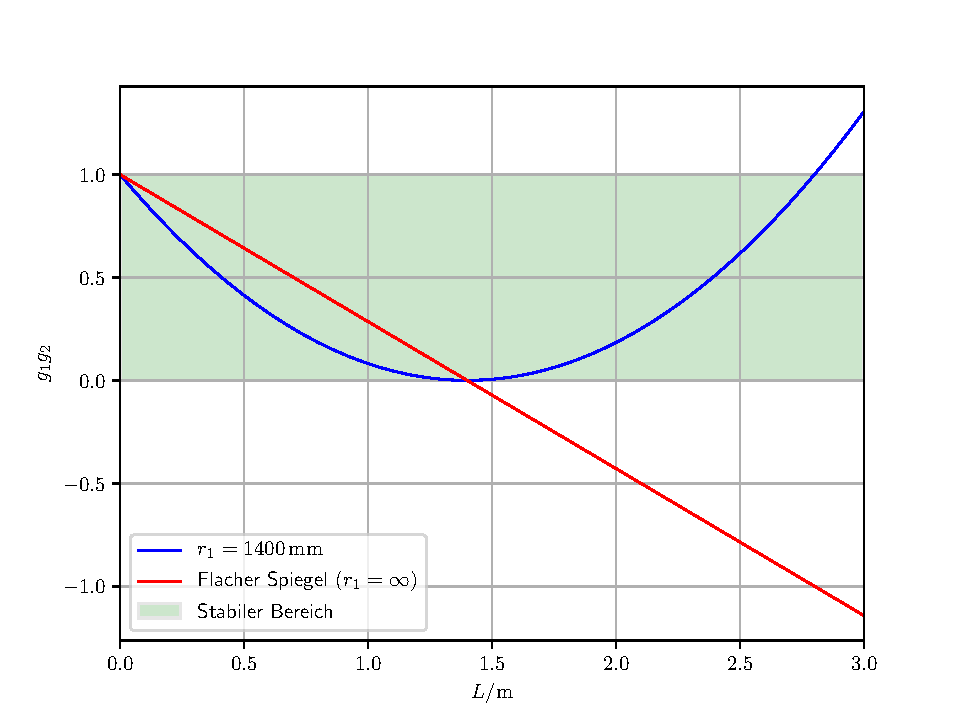
\includegraphics[width = \textwidth]{Pics/g_1_g_2.pdf}
  \caption{Verlauf des Stabilitätsparameters. \cite{StevenStefan}}
  \label{fig:g1g2}
\end{figure}

\subsection{Elektromagnetische Moden des Lasers}

Im Allgemeinen ist die Resonatorlänge deutlich größer als die Wellenlänge $\lambda$
des emittierten Lichtes. Somit können mehrere Moden auftauchen. Die Anzahl q der
Wellenlängen im Resonator wird als longitudinale Mode bezeichnet. Aufgrund von
Unebenheiten der Spiegeloberflächen tuach zusätzliche transversale Moden auf,
die im folgenden als $TEM\ua{lp}$ (transverse electromagnetic mode) bezeichnet werden.
Bei l handelt es sich dabei um die Anzahl der auftretenden Knoten in x-Richtung und bei p
dementsprechend um die Anzahl  der Knoten in y-Richtung. Da höhere Moden auch
höhere Verluste erzeugen, sind im Resonator nur wenige transversale Moden stabil
und werden verstärkt.
